\documentclass[a4paper,12pt]{report}

\usepackage[utf8]{inputenc}
\usepackage[francais]{babel}
\usepackage{graphicx}
\usepackage{fancyhdr}
\usepackage[absolute]{textpos}
\usepackage[svgnames]{xcolor}
\usepackage{colortbl}
\usepackage{lastpage}
\usepackage{url}
\usepackage[hidelinks]{hyperref}
\usepackage{geometry}
\usepackage{tikz}
\usepackage{titlesec}
\usepackage{datetime}
\usepackage{lipsum}
\usepackage{array}
\usepackage{supertabular}
\usepackage{float}
\usetikzlibrary{matrix}

\newcommand{\doctitle}{WBS}
\newcommand{\doclongtitle}{Work Breakdown Structure}

\title{\doctitle{} Vigilitate}
\author{Soules Kévin, Mercier Daniel, Budowski Prune, Harscoat Morgane, Poncet Manuel, Keller Flavien}
\date{\today}


\definecolor{myBlue}{RGB}{23,54,93}
\definecolor{lightGray}{gray}{0.7}
\newdateformat{slashdate}{\twodigit{\THEDAY}/\twodigit{\THEMONTH}/\THEYEAR}
\newcolumntype{R}[1]{>{\centering\let\newline\\\arraybackslash\hspace{0pt}}m{#1}}

\titleformat{\section}[block]{\bfseries}{\thesection.}{1em}{}
\titleformat{\subsection}[block]{\hspace{2em}}{\thesubsection}{1em}{}
\titleformat{\subsubsection}[block]{\hspace{3em}}{\thesubsubsection}{1em}{}
  
\geometry{
  a4paper,
  left=20mm,
  right=20mm,
}

\setlength{\unitlength}{1mm}
\addtolength{\headheight}{1.5\baselineskip}
\renewcommand{\headrulewidth}{0.0pt}
\renewcommand{\footrulewidth}{0.4pt}


\fancypagestyle{eip}{
  \fancyhf{}
  \fancyhead[L] {
    \includegraphics[width=3cm]{../../logos/logo_eip.png}
  }
  \fancyhead[R] {
    \colorbox{myBlue}{
      \textcolor{white}{
        \Large \textbf{[2017][Vigilate][\doctitle{}]}
      }
    }
  }
  \renewcommand{\headrulewidth}{0pt}
  \fancyfoot[L]{
    \textcolor{gray}{
      \{EPITECH.\}
    }
  }
  \fancyfoot[C]{}
  \fancyfoot[R]{
    \ifnum\value{page}>0
    \thepage/\pageref{LastPage}
    \fi
  }
}

\makeatletter
\let\ps@plain\ps@eip
\makeatother

\pagestyle{eip}


\begin{document}
\date{\slashdate\today}
\setcounter{page}{-10}

% --- (1) Page de garde ---

\thispagestyle{empty}
\vspace*{\stretch{2}}
\begin{center}
  \textcolor{myBlue}{\Huge \textbf{EIP Vigilitate}}\linebreak
  \vspace*{\stretch{1}}
  \textcolor{gray}{\textit{\Large \doclongtitle{} (\doctitle{})}}\linebreak
  \vspace*{\stretch{1}}
  {\today}
\end{center}
\vspace*{\stretch{1}}
\newpage

% --- (2) Résumé ---

\vspace*{\stretch{1}}
\begin{flushleft}
  \textcolor{myBlue}{\textit{\large \textbf{Résumé du document}}}\linebreak
\end{flushleft}
Le cahier des charges commence par un bref rappel de notre EIP, Vigilate, un outil de sécurité informatique qui permet de se tenir informé des dernières vulnérabilités publiques rapidement sur tous les programmes que l’utilisateur souhaite vérifier. On mettra en avant les contraintes fonctionnelles et les exigences non-fonctionnelles comme le fait que notre projet doit être sécurisé, ou alors la réactivité de notre outil. Notre projet est réalisé par 6 personnes. Le document présente d’une part la structure du projet : un site web, le back-end, une machine virtuelle et un scanneur de programme et d’autre part, les différentes fonctionnalités du projet à partir d’un document UML (connexion de l’utilisateur, possibilité de modifier ses préférences : programmes à surveiller, style d’alerte souhaité...). Nous présentons dans la partie 6 l’organisation prévue : 2 personnes sur le site web, 2 sur le back-end, 1 sur la machine virtuelle et 1 sur le scanneur de programme. Ainsi que la méthodologie utilisée, basée sur la méthode Agile (Scrum). Pour ce faire, nous devons construire un produit backlog avant de commencer à développer le projet, puis organiser un nombre de sprints adéquat, d’une durée relativement courte (principe de la méthode agile) mais qui permettront d’avoir un projet fonctionnel à chaque fin de sprint avec chaque tâche décrite dans un backlog de sprint. Nous présenterons également l’environnement et les outils utilisés (github pour héberger nos documents...). Nous avons réalisé un template de mise en page pour toute notre documentation avec Latex. Nous avons choisi de respecter la norme Python Pep8 pour le développement. Dans une dernière partie, nous proposerons une description des tests, utilisés pendant le développement notamment grâce à l’outil Travis et les tests une fois l’outil terminé.\\
\vspace*{\stretch{1}}
\newpage

% --- (3) Cartouche + révisions ---

\begin{flushleft}
  \vspace*{\stretch{1}}
  \textcolor{myBlue}{\textit{\large \textbf{Description du document}}} 
  \bigbreak
  \begin{tabular}{|>{\columncolor[RGB]{220,220,220}\color{Navy}\bfseries}l|p{12cm}|}
\hline
Titre & [2017][Vigilate][\doctitle{}] \\
\hline
Date & 31/01/2015 \\
\hline
Auteur & Kévin SOULES \\
\hline
Responsable & Kévin SOULES\\
\hline
Email & vigilate\_2017@labeip.epitech.eu\\
\hline
Sujet & \doclongtitle{}\\
\hline
Mots clés & \doctitle{}, sécurité, vulnérabilités\\
\hline
Version du modèle & 1.1\\
\hline
\end{tabular}


  \vspace*{\stretch{2}}
  \bigbreak
  \bigbreak
  \textcolor{myBlue}{\textit{\large \textbf{Tableau des révisions}}}
  \bigbreak
  \small
\begin{tabular}{|p{1.5cm}|l|p{2.5cm}|p{7.8cm}|l|}
  \hline
 
   \rowcolor{Gainsboro}Date  & Auteur & Section(s) & Commentaires \\
  \hline
24/01/15 & Kévin Soules &  & Création du documents\\
  \hline
27/01/15 & Kévin Soules & Chapitre 1 et 2.1 & Recherche de liste de solutions. Rédaction du texte d'un premier concurrent. Remplissage des rappels.\\
\hline
28/01/15 & Prune Budowski & Chapitre 1 & Amélioration des rappels \\
\hline
29/01/15 & Prune Budowski & Chapitre 3.3.2 & Rédaction de la partie ``Ce qui ne sera pas couvert''\\
\hline
29/01/15 & Daniel Mercier & Chapitre 2.2 & Rédaction du texte du deuxième concurrent.\\
\hline
29/01/15 & Kévin Soules & Chapitre 2.3 & Rédaction du texte du troisième concurrent. \\
\hline
30/01/15 & Morgane Harscoat & Chapitre 2.4 & Début de rédaction du texte du quatrième concurrent. \\
\hline
30/01/15 & Kévin Soules & Chapitre 2.5 & Rédaction du texte du cinquième concurrent.\\
\hline
31/01/15 & Kévin Soules & Conclusion, Glossaire & Matrice de préférence.Rédaction d'un glossaire. \\
\hline
31/01/15 & Prune Budowski & Résumé, Conclusion, Chapitre 3.1 & Rédaction du résumé. SWOT. Rédaction de la partie ``Ce que vous apportez''.  
  \\
\hline
31/01/15 & Daniel Mercier & Toutes & Corrections. \\
31/01/15 & Prune Budowski & & Mise en page. \\
31/01/15 & Kévin Soules & & Mise en page.
\\
  \hline
\end{tabular}
\normalsize

  \vspace*{\stretch{1}}
\end{flushleft}

% --- (4) Tables des matières ---

\tableofcontents

% --- (5) Rappel eip ---

\textcolor{myBlue}{\chapter{Rappel de l'EIP}}
\setcounter{page}{1}
\section{Qu'est-ce qu’un EIP et Epitech}
Epitech,  école de l'innovation et de l'expertise informatique propose un cursus en 5 années, basé sur une pédagogie par projet (à réaliser seul ou en groupe). L'un de ces projets, l’EIP (Epitech Innovating Project), réalisé par groupes de 6 à 15 étudiants, démarre au cours de la 3\ieme année et se déroule sur 2 ans et demi. Ce  projet doit être particulièrement innovant, car son objectif est d’être commercialisable à la fin de la 5\ieme année d’Epitech.

\section{Sujet de votre EIP}
Le but de Vigilate est d’avertir les utilisateurs des services obsolètes ou potentiellement vulnérables affectant en particulier leur infrastructure (sites web, réseau d'entreprises, logiciels), dans le but de les informer des risques techniques encourus et des éventuelles mises à jour ou corrections à appliquer.
Cela sans effectuer de scan de vulnérabilité.
Nous proposons cependant un outil de scan de programme qui envoie la liste sur notre plateforme web.

\section{Glossaire}
\noindent
\vskip 0.1cm
\textbf{- C -}\\
\vskip 0.1cm
\textit{CVE (Common Vulnerabilities and Exposures)}: dictionnaire d'informations publiques relatives aux vulnérabilités informatiques. Par métonymie, on emploie souvent le terme CVE à la place de CVE ID (ou identifiant CVE), qui lui désigne le numéro qui renvoie à la fiche descriptive complète de cette vulnérabilité. Exemple: CVE-2013-4343.\\
\textit{CSIRT (Computer Security Incident Response Team)}: équipe chargée d'assurer la sécurité d'une entreprise.\\
\textit{CERT (Computer Emergency Response Team)}: marque déposée représentant les CSIRT certifiés.\\
\vskip 0.1cm
\textbf{- F -}\\
\vskip 0.1cm
\textit{Fingerprint}: déduction de la version d'un programme/système d'exploitation en fonction de la façon dont il répond à nos requêtes sur le réseau.\\
\textit{Fork}: création d'un nouveau programme en utilisant le code source du premier.\\
\vskip 0.1cm
\textbf{- G -}\\
\vskip 0.1cm
\textit{GPL (General Public License)}: licence dédiée aux logiciels libres.\\
\vskip 0.1cm
\textbf{- P -}\\
\vskip 0.1cm
\textit{Patch}: un correctif qui corrige un bug ou une vulnérabilité dans un programme.\\
\vskip 0.1cm
\textbf{- S -}\\
\vskip 0.1cm
\textit{SCADA (Supervisory Control and Data Acquisition)}: système de télégestion à grande échelle utilisé dans l'industrie.\\




\chapter{Contexte}
\section{Hypothèses}
La partie backend sera développée en python. Un langage simple, rapide à écrire et performant.\\
Le site web utilisera le framwork django et son frontend sera développé avec angular js\\
Le programme de scan sera développé en python ce qui permettra une portabilité aisée.\\
La distribution présente sur la vm sera une debian. Ce qui permettra d’avoir une stabilité reconnue dans le temps.\\

\section{Contraintes}
L’interface utilisateur devra être intuitive et facile d’utilisation pour l’utilisateur lambda, dans le but de favoriser un maximum l’accès à nos services en toute simplicité.\\
La réactivité sera un des points principaux à respecter afin de ne laisser s’échapper qu’un minimum de temps entre la diffusion d’une CVE et sa transmission aux clients concernés.\\
Être sécurisé afin d’éviter impérativement une potentielle fuite d’informations relative aux clients ou à notre infrastructure.\\


\let\clearpage\relax
\vspace*{0.8cm}
\hspace*{-1cm}
\textcolor{myBlue}{\chapter{WBS}}
\section{Représentation du WBS}

\hspace*{-2cm}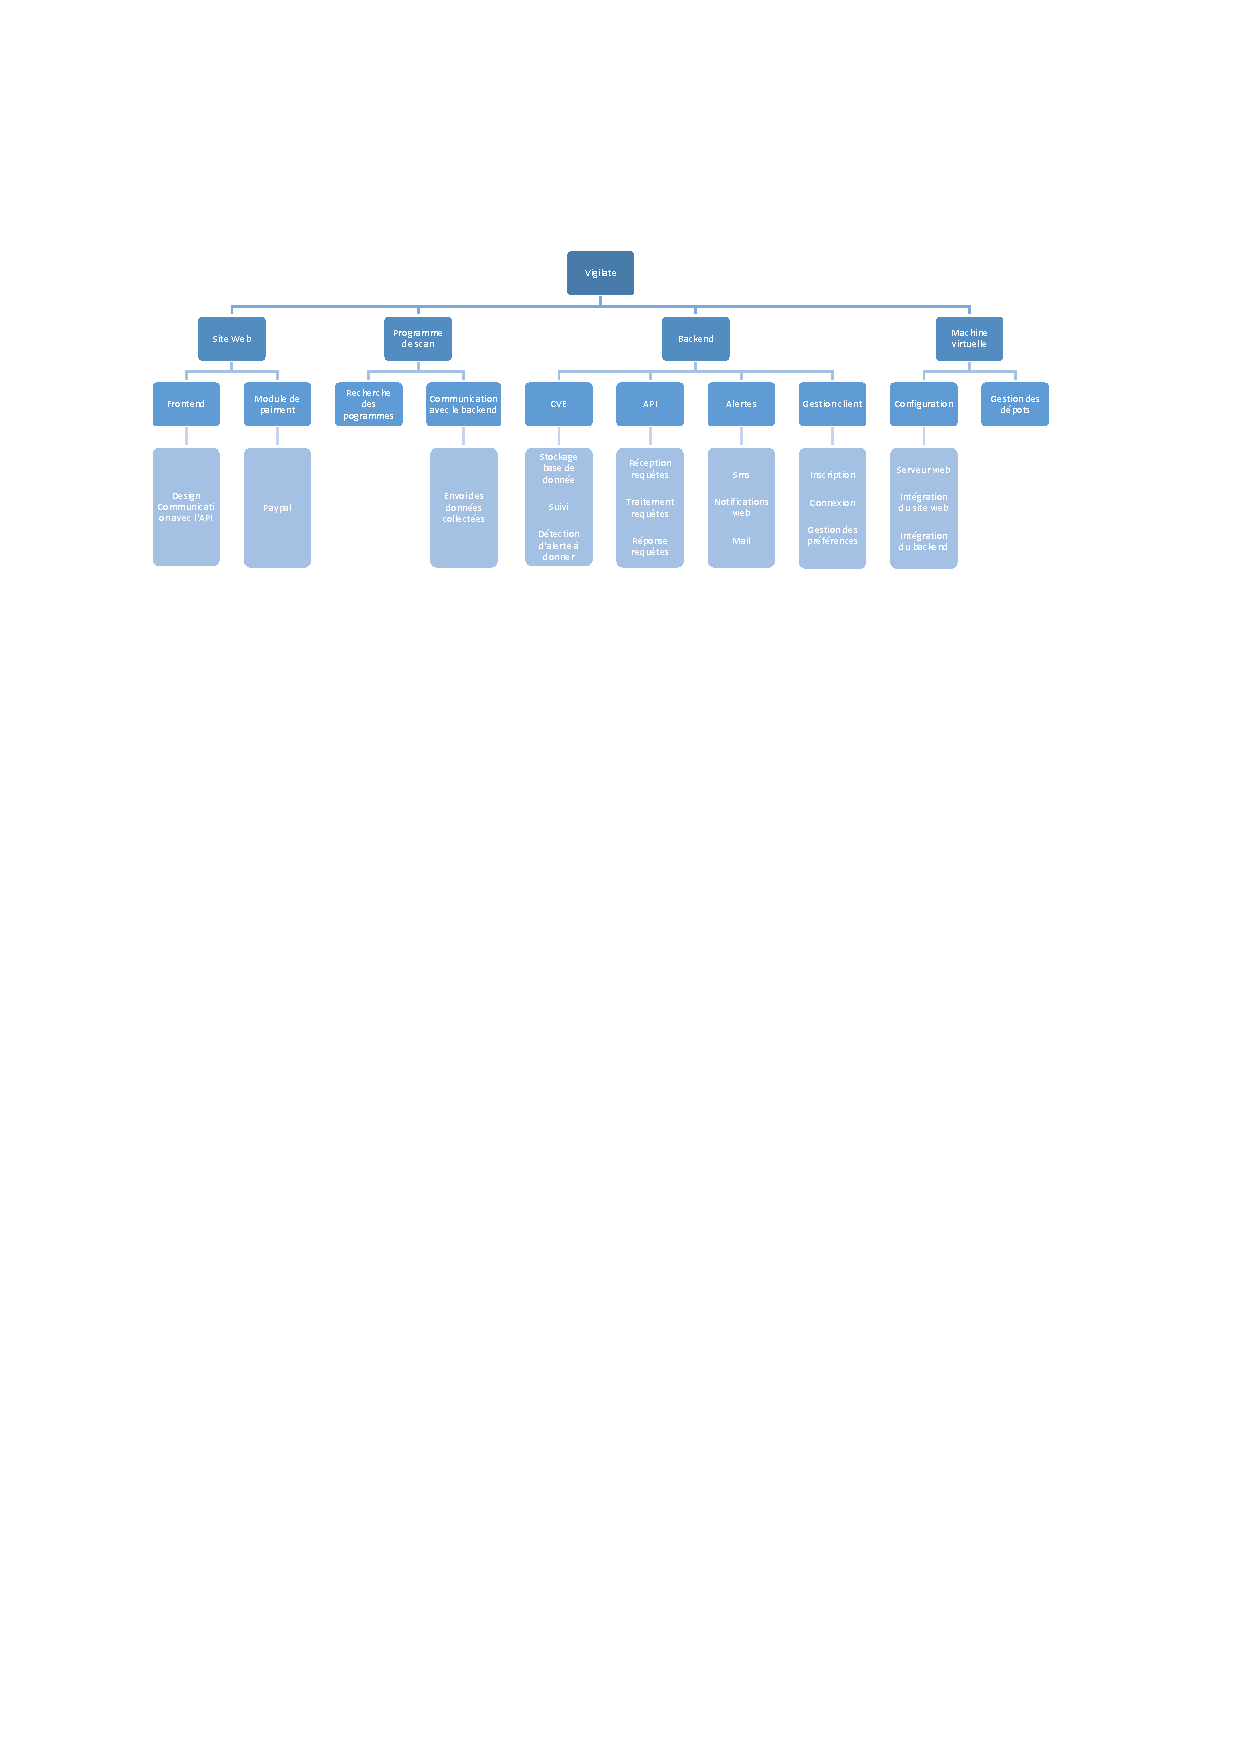
\includegraphics[trim = 2.5cm 0 0 3cm, clip, width=23.9cm]{Organigramme.pdf}
\section{Dictionnaire du WBS}
\footnotesize
\begin{supertabular}{|p{1.5cm} p{6cm}|p{5cm}|R{2cm}|}
  \hline
  \rowcolor{myBlue}
  \textcolor{white}{\textbf{ID}} & \textcolor{white}{\textbf{Fonctionnalité}} & \textcolor{white}{\textbf{Description}} & \textcolor{white}{\textbf{\% réalisé}} \\
  \hline
  \hline

  % Site Web

  \rowcolor{myBlue}
  \textcolor{white}{\textbf{1}} & \textcolor{white}{\textbf{Site Web}} & \textcolor{white}{\textbf{Réaliser le site web}} & \textcolor{white}{\textbf{0\%}} \\
  \hline

  \rowcolor{lightGray}
  \textbf{1.1}  & \textbf{Frontend} & \textbf{Réaliser la partie frontal} & \textbf{0\%} \\
  \hline

  \hspace{6pt}
  \textbf{1.1.1}  & \textbf{Design} & Réaliser le design du site & 0\% \\
  \hline

  \hspace{6pt}
  \textbf{1.1.2}  & \textbf{Communication avec l'API} & Réaliser la partie qui communique avec l'API & 0\% \\
  \hline


  \rowcolor{lightGray}
  \textbf{1.2}  & \textbf{Module de paiement} & \textbf{Intégration d'un module de paiement} & \textbf{0\%} \\
  \hline

  \hspace{6pt} \textbf{1.2.1}  & \textbf{Paypal} & Intégration de paypal & 0\% \\
  \hline


  % Programme de scan


  \rowcolor{myBlue}
  \textcolor{white}{\textbf{2}}  & \textcolor{white}{\textbf{Programme de scan}} & \textcolor{white}{\textbf{Réaliser un programme de scan}} & \textcolor{white}{\textbf{0\%}} \\
  \hline

  \rowcolor{lightGray}
  \textbf{2.1}  & \textbf{Recherche des programmes} & \textbf{Réaliser la partie recherche de programme} & \textbf{0\%} \\
  \hline

  \rowcolor{lightGray}
  \textbf{2.2}  & \textbf{Communication avec le backend} & \textbf{Réaliser la partie qui communique avec le backend} & \textbf{0\%} \\
  \hline

  \hspace{6pt}
  \textbf{2.2.1}  & \textbf{Envoi des données collectées} & Envoi des données au backend & 0\% \\
  \hline

  % Backend

  \rowcolor{myBlue}
  \textcolor{white}{\textbf{3}}  & \textcolor{white}{\textbf{Backend}} & \textcolor{white}{\textbf{Réaliser un backend}} & \textcolor{white}{\textbf{0\%}} \\
  \hline

  \rowcolor{lightGray}
  \textbf{3.1}  & \textbf{CVE} & \textbf{Réaliser la partie qui gère les CVE} & \textbf{0\%} \\
  \hline

  \hspace{6pt}
  \textbf{3.1.1}  & \textbf{Stockage en bdd} & Stockage en bdd des CVE reçus & 0\% \\
  \hline

  \hspace{6pt}
  \textbf{3.1.2}  & \textbf{Suivi} & Suivre en permanence la sortie des nouvelles CVE  & 0\% \\
  \hline

  \hspace{6pt}
  \textbf{3.1.3}  & \textbf{Détection d'alerte à donner} & Réaliser une partie qui va être lancé à chaque nouvelle CVE afin de détecter à qui il faut envoyer une alerte & 0\% \\
  \hline


  \rowcolor{lightGray}
  \textbf{3.2}  & \textbf{API} & \textbf{Réaliser l'API} & \textbf{0\%} \\
  \hline

  \hspace{6pt}
  \textbf{3.2.1}  & \textbf{Réception requêtes} & Réaliser la partie qui reçoit les requêtes & 0\% \\
  \hline

  \hspace{6pt}
  \textbf{3.2.2}  & \textbf{Traitement des requêtes} & Réaliser la partie qui traite les requêtes  & 0\% \\
  \hline

  \hspace{6pt}
  \textbf{3.2.3}  & \textbf{Réponse au requêtes} & Réaliser la partie qui répond au reuqêtes & 0\% \\
  \hline


  \rowcolor{lightGray}
  \textbf{3.3}  & \textbf{Alertes} & \textbf{Réaliser la partie qui gère les alertes} & \textbf{0\%} \\
  \hline

  \hspace{6pt}
  \textbf{3.3.1}  & \textbf{SMS} & Réaliser un module d'alerte SMS  & 0\% \\
  \hline

  \hspace{6pt}
  \textbf{3.3.2}  & \textbf{Notification web} & Réaliser un module d'alerte via l'interface du site web & 0\% \\
  \hline

  \hspace{6pt}
  \textbf{3.3.3}  & \textbf{Mail} & Réaliser un module d'alerte SMS & 0\% \\
  \hline


  \rowcolor{lightGray}
  \textbf{3.4}  & \textbf{Gestion utilisateurs} & \textbf{Réaliser la partie qui gère les utilisateurs} & \textbf{0\%} \\
  \hline

  \hspace{6pt}
  \textbf{3.4.1}  & \textbf{Inscription} & Réaliser une partie inscription & 0\% \\
  \hline

  \hspace{6pt}
  \textbf{3.4.2}  & \textbf{Connexion} & Réaliser une partie connexion & 0\% \\
  \hline

  \hspace{6pt}
  \textbf{3.4.3}  & \textbf{Gestion préférences} & Réaliser une partie de gestion de préférence & 0\% \\
  \hline



  % VM


  \rowcolor{myBlue}
  \textcolor{white}{\textbf{4}}  & \textcolor{white}{\textbf{Machine virtuelle}} & \textcolor{white}{\textbf{Réaliser une vm}} & \textcolor{white}{\textbf{0\%}} \\
  \hline

  \rowcolor{lightGray}
  \textbf{4.1}  & \textbf{Configuration} & \textbf{Configurer la vm} & \textbf{0\%} \\
  \hline

  \hspace{6pt}
  \textbf{4.1.1}  & \textbf{Serveur web} & Configurer un serveur web & 0\% \\
  \hline

  \hspace{6pt}
  \textbf{4.1.2}  & \textbf{Intégration site web} & Intégrer le site web sur la vm & 0\% \\
  \hline

  \hspace{6pt}
  \textbf{4.1.3}  & \textbf{Intégration backend} & Intégrer le backend sur la vm & 0\% \\
  \hline


  \rowcolor{lightGray}
  \textbf{4.2}  & \textbf{Dépots} & \textbf{Gestion des dépots} & \textbf{0\%} \\
  \hline



\end{supertabular}
\normalsize



\end{document}